\documentclass{beamer}
%\documentclass[handout]{beamer}
\usepackage{caption}
\usepackage{natbib}
\usepackage{cite}
\usepackage{graphicx}
\usepackage{tikz}
\usepackage{verbatim}
\usepackage{listings}
\usecolortheme[dark]{solarized}
\title{User Study of Tools to Assist Java Programmers in Finding Bugs}
\author[Landgrebe]{Andreas Bach Landgrebe}
\institute[Allegheny College]{Department of Computer Science \\ Allegheny College}
\date{\today}

\lstset{frame=tb,
  language=Java,
  aboveskip=3mm,
  belowskip=3mm,
  showstringspaces=false,
  columns=flexible,
  basicstyle={\small\ttfamily},
  numbers=none,
  %numberstyle=\tiny\color{gray},
  %keywordstyle=\color{blue},
  %commentstyle=\color{dkgreen},
  %stringstyle=\color{mauve},
  breaklines=true,
  breakatwhitespace=true,
  tabsize=3
}


\usetikzlibrary{calc,trees,positioning,arrows,chains,shapes.geometric,%
    decorations.pathreplacing,decorations.pathmorphing,shapes,%
    matrix,shapes.symbols}
\tikzset{
>=stealth',
  punktchain/.style={
    rectangle, 
    rounded corners, 
    % fill=black!10,
    draw=orange, very thick,
    text width=10em, 
    minimum height=1em, 
    text centered, 
    on chain},
  line/.style={draw, thick, <-},
  element/.style={
    tape,
    top color=white,
    bottom color=blue!50!black!60!,
    minimum width=8em,
    draw=blue!40!black!90, very thick,
    text width=10em, 
    minimum height=1em, 
    text centered, 
    on chain},
  every join/.style={->, thick,shorten >=1pt},
  decoration={brace},
  tuborg/.style={decorate},
  tubnode/.style={midway, right=2pt},
}

\begin{document}

\begin{frame}
  \titlepage
\end{frame}




\begin{frame}
\frametitle{Motivation}
\framesubtitle{Wrong Poker Representation}
\begin{center}
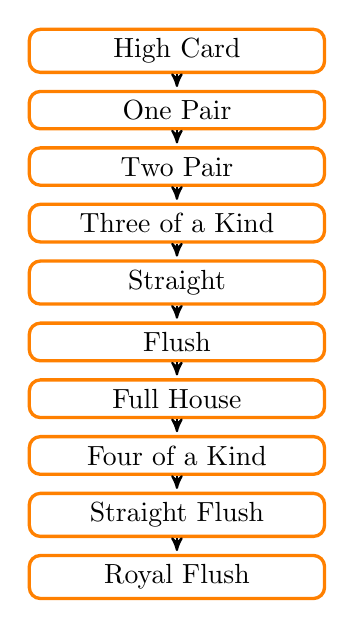
\begin{tikzpicture}
  [node distance=.2cm,
  start chain=going below,]
     \node[punktchain, join](HighCard){High Card};
     \node[punktchain, join](OnePair){One Pair};
     \node[punktchain, join](TwoPair){Two Pair};
     \node[punktchain, join](ThreeofaKind){Three of a Kind};
     \node[punktchain, join](Straight){Straight};
     \node[punktchain, join](Flush){Flush};
     \node[punktchain, join] (FullHouse){Full House};
     \node[punktchain, join] (FourofaKind){Four of a Kind};
     \node[punktchain, join] (StraightFlush){Straight Flush};
     \node[punktchain, join] (RoyalFlush) {Royal Flush}; 
   \end{tikzpicture}
   \end{center}
\end{frame}

\begin{frame}
\frametitle{Motivation}
\framesubtitle{Correct Poker Representation}
\begin{center}
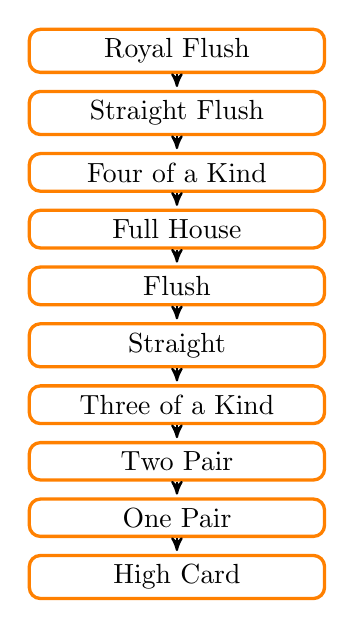
\begin{tikzpicture}
  [node distance=.2cm,
  start chain=going below,]
     \node[punktchain, join] (RoyalFlush) {Royal Flush};
     \node[punktchain, join] (StraightFlush){Straight Flush};
     \node[punktchain, join] (FourofaKind){Four of a Kind};
     \node[punktchain, join] (FullHouse){Full House};
     \node[punktchain, join](Flush){Flush};
     \node[punktchain, join](Straight){Straight};
     \node[punktchain, join](ThreeofaKind){Three of a Kind};
     \node[punktchain, join](TwoPair){Two Pair};
     \node[punktchain, join](OnePair){One Pair};
     \node[punktchain, join](HighCard){High Card};
  % Now that we have finished the main figure let us add some "after-drawings"
  %% First, let us connect (finans) with (disk). We want it to have
  %% square corners. 
   \end{tikzpicture}
   \end{center}
\end{frame}

\begin{frame}
\frametitle{Motivation}
\framesubtitle{Definitions}
\begin{itemize}
\item<1-> Logic Bug: is a bug in a program that causes it to operate incorrectly but not to terminate or crash.
\item<2-> Static Program Analysis: analysis of computer software that is performed without actually executing programs.
\item<2-> Dynamic Program Analysis: analysis of computer software that is performed by executing programs on a real or virtual processor.
\end{itemize}
\end{frame}

\begin{frame}
\frametitle{Motivation}
\framesubtitle{Why I decided this project}
\begin{itemize}
\item<1-> Logic errors are the most difficult to find and fix.
%other type of bugs include run-time errors and compiler errors
\item<2-> There is not one tool that will do everything for the programmer.
\item<3-> These three tools are the most popular pieces of software when looking for logic-based bugs in Java.
\end{itemize}
\end{frame}



\begin{frame}
\frametitle{Overview of Project}
\begin{itemize}
\item<1-> Three Static Code Analysis Tools
\item<1-> Evaluate each of these three tools and provide an evaluation on how each tool operates.
\item<2-> Eclipse Integrated Development Environment
\begin{itemize}
\item<3-> Findbugs
\item<4-> PMD
\item<5-> checkstyle
\end{itemize}
\item<6-> Implementation of five Java files with buggy code.
\item<7-> Human Study starting with students of Computer Science 112.
\end{itemize}
\end{frame}

\begin{frame}
\frametitle{Tools}
\framesubtitle{Findbugs}
\centering
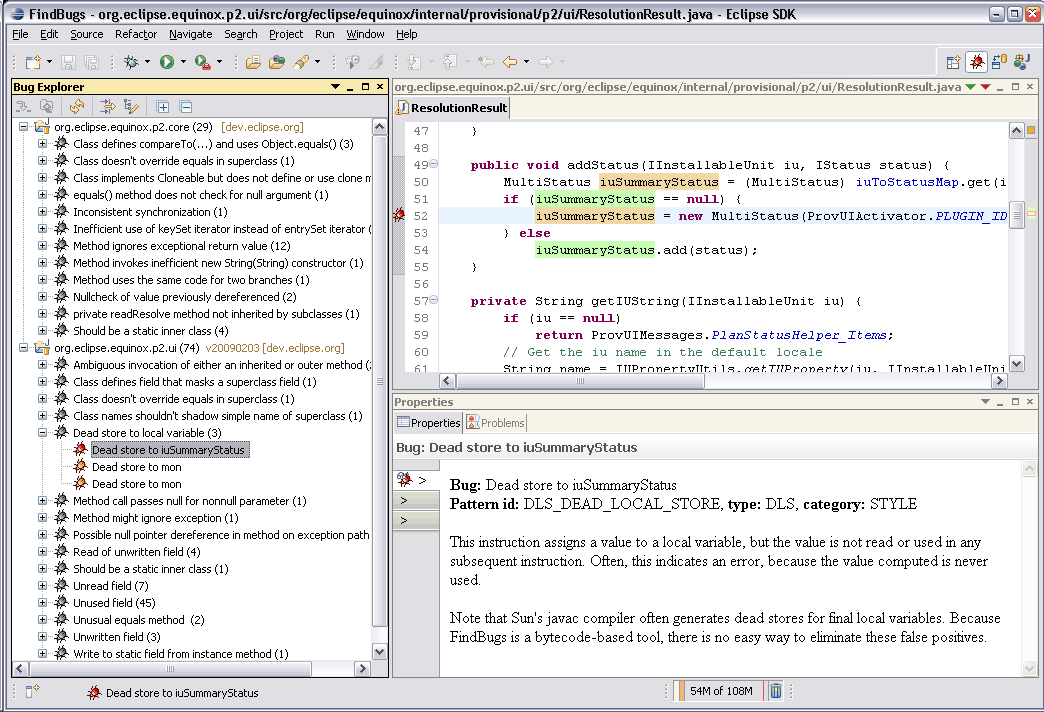
\includegraphics[scale=0.3]{findbugs_1}
\end{frame}


\begin{frame}
\frametitle{Tools}
\framesubtitle{Features of FindBugs}
\begin{itemize}
\item<1-> Operates on Java bytecode
\item<2-> Additional rule sets can be plugged in.
\item<3-> Bugs Rank 1-20
\begin{itemize}
\item<4-> Rank 1-4: Scariest
\item<5-> Rank 5-9: Scary
\item<6-> Rank 10-14: Troubling
\item<7-> Rank 15-20: Concern
\end{itemize}
\end{itemize}
\end{frame}

\begin{frame}
\begin{figure}
\frametitle{Tools}
\framesubtitle{PMD}

\includegraphics[width=0.1\textwidth]{pmd_logo}
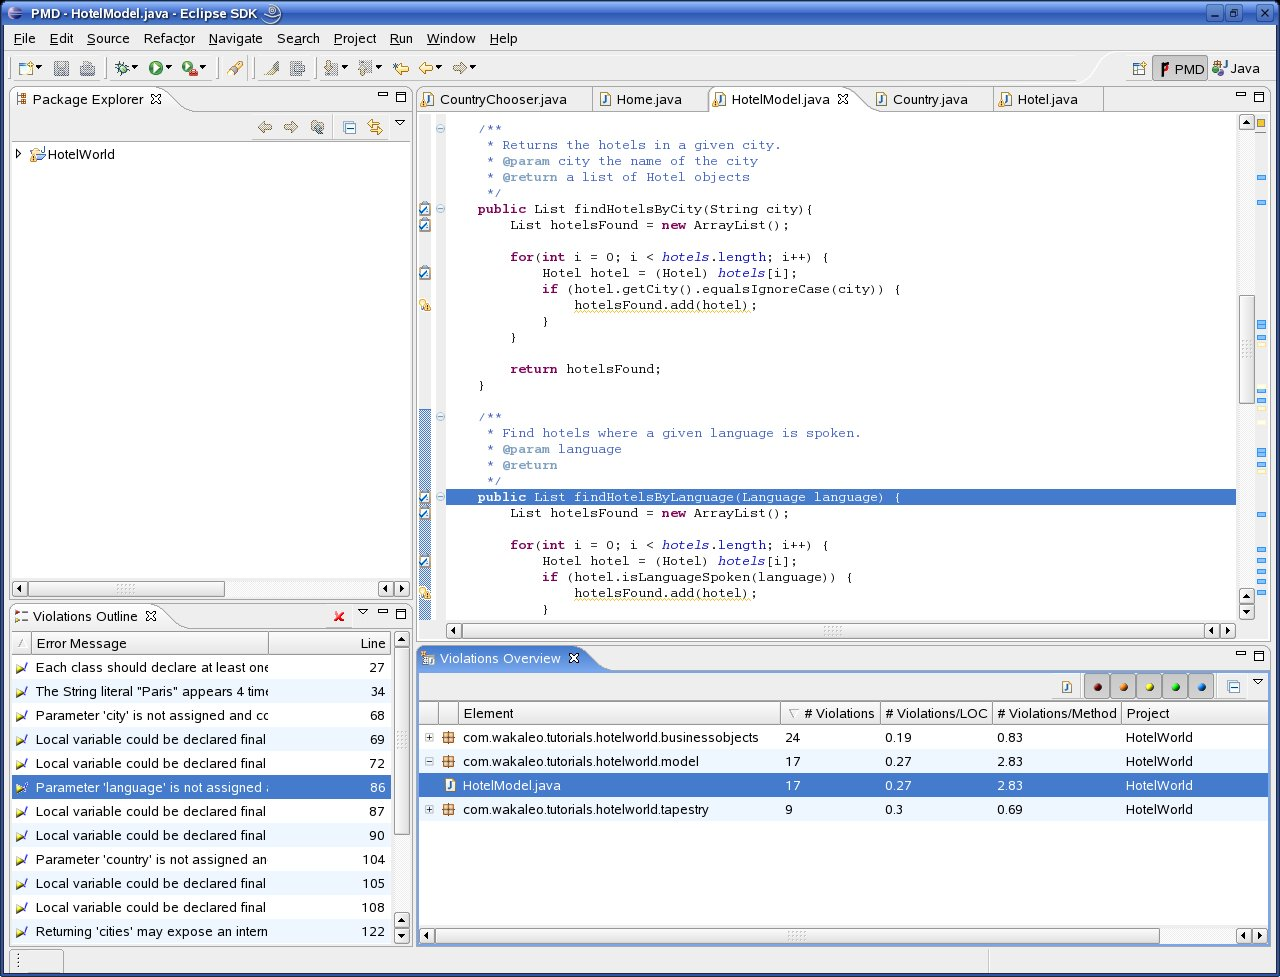
\includegraphics[width=0.9\textwidth]{PMD_eclipse.jpg}
\end{figure}
\end{frame}

\begin{frame}
\frametitle{Tools}
\framesubtitle{PMD}
\begin{itemize}
\item<1-> Java source code analyzer
\item<2-> Built-in rules and supports the ability to write custom rules
\item<3-> Not true errors, but rather inefficient code
\begin{itemize}
\item<1-> PMD possible flaws to detect
\begin{itemize}
\item<2-> Possible bugs - Empty try/catch/switch blocks.
\item<3-> Dead code - Unused variables and private methods.
\item<4-> Empty if/while statements
\item<5-> Overcomplicated expressions - for loops that could be while loops
\item<6-> Suboptimal code - Wasteful String usage
\item<7-> Classes with high Cyclomatic Complexity measurements (complexity of a program).
\item<8-> Duplicated code - copied-pasted code could mean copied/pasted bugs.
\end{itemize}
\end{itemize}
\end{itemize}
\end{frame}


\begin{frame}
\frametitle{Tools}
\framesubtitle{Checkstyle}

\includegraphics[width=0.1\textwidth]{header-checkstyle-logo}
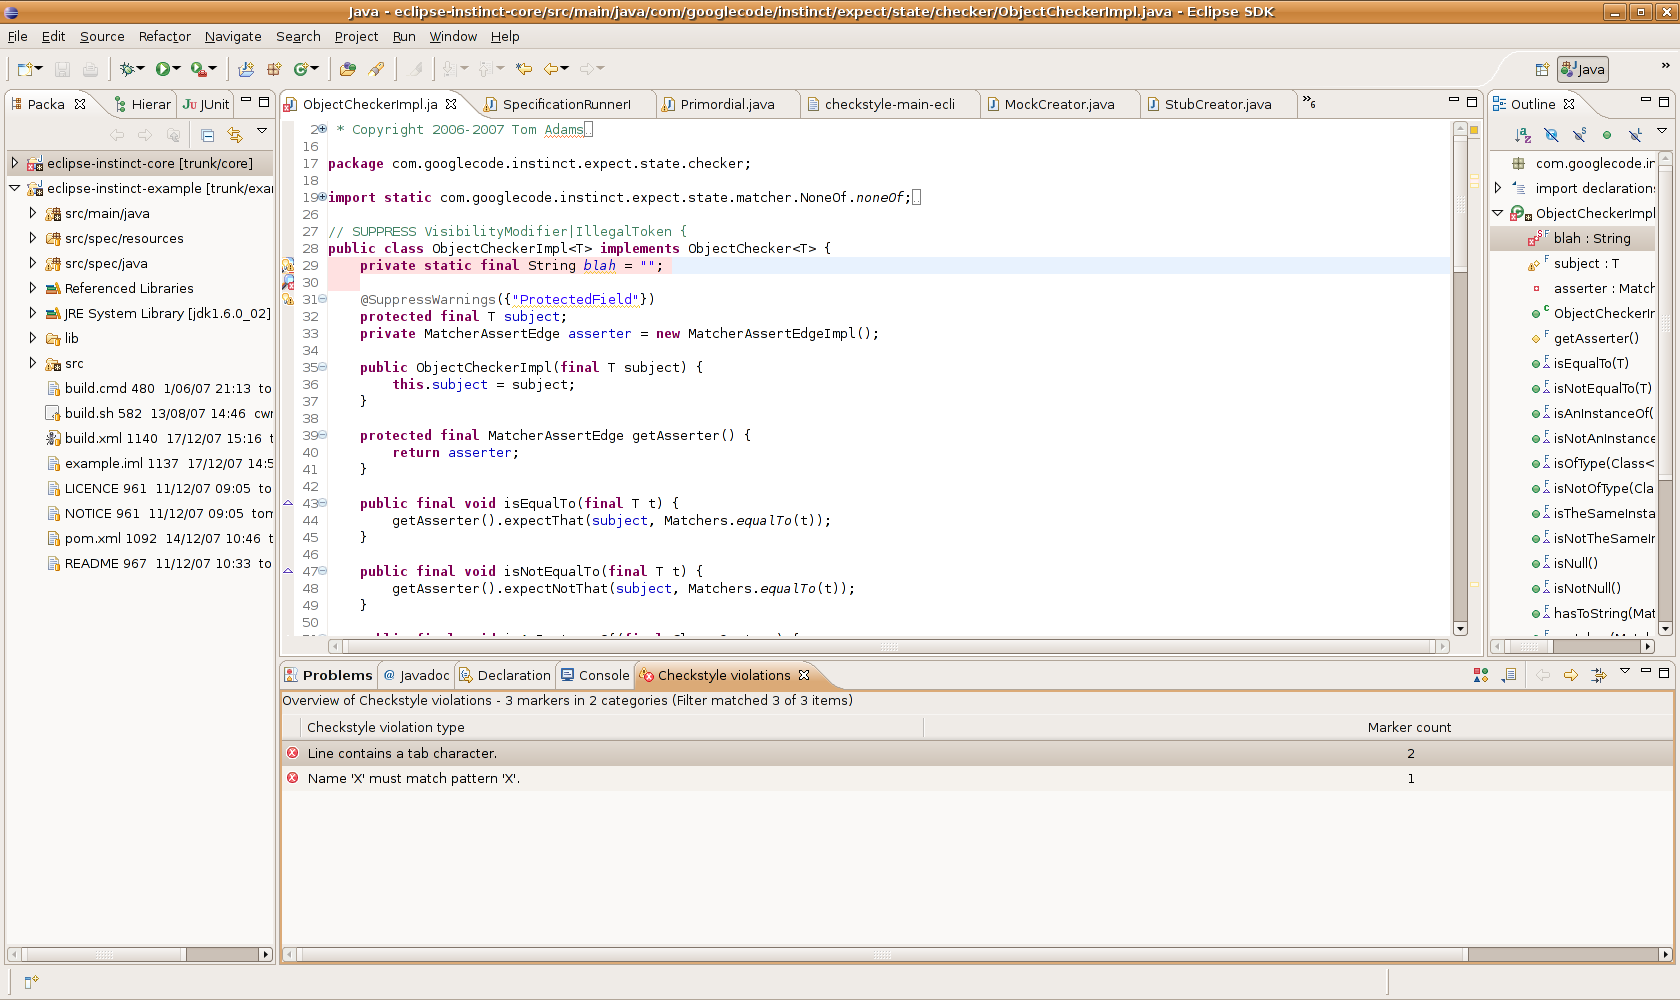
\includegraphics[width=0.9\textwidth]{Eclipse_Checkstyle_Sample_Error}
\end{frame}

\begin{frame}
\frametitle{Tools}
\framesubtitle{Checkstyle}
\begin{itemize}
\item<1-> Java source code analyzer
\item<2-> Checks if Java source code adheres to a coding standard
\item<3-> Highly configurable to support any coding standard
\item<4-> Designed to check for programming practices.
%examples of this: instead of error reporting, system.exit 
\end{itemize}
\end{frame}


\begin{frame}
\frametitle{Evaluation Strategy}
\begin{itemize}
\item<1-> Five Java programs with logic-based bugs
\begin{itemize}
\item<2-> Misplaced semi-colon
\item<3-> Velocity logic-bug
\item<4-> String == vs. String equals() comparison bug
\item<5-> Memory leak bug
\item<6-> Switch case bug
\end{itemize}
\end{itemize}
\end{frame}

\begin{frame}
\frametitle{Evaluation Strategy}
\framesubtitle{Human Study Survey}
\begin{itemize}
\item<1-> Did you find the bugs?
\item<2-> If yes, did Findbugs assist you in finding these bugs?
\item<3-> If yes, did PMD assist you in finding these bugs?
\item<4-> If yes, did Checkstyle assist you in finding these bugs
\item<5-> Would you use any of these tools in the future for finding logic-based bugs?
\item<6-> Suggestion to further improve these tools.
\end{itemize}
\end{frame}

\begin{frame}
\frametitle{Evaluation Strategy}
\framesubtitle{How To Evaluate Human Study}
\begin{itemize}
\item<1-> Computer Science 112 Students
\item<2-> Knowledge past Computer Science 111
\item<3-> 24 hours to evaluate and find the logic bugs
\item<4-> IRB approval and CITI Training
\end{itemize}
\end{frame}



\begin{frame}
\frametitle{Deliverables}
\begin{itemize}
\item<1-> Evaluation of how each of these three tools operates.
\item<2-> User study of whether these three tools assisted in finding these bugs.
\item<3-> Human Study of whether these three tools were able to help Java programmers finding logic bugs.
\item<4-> Java source code with logic-based bugs
\end{itemize}
\end{frame}


\begin{frame}
\frametitle{Conclusion}
\framesubtitle{Thank You!}
Comments, Questions or Concerns?
\end{frame}
\end{document}